% Written by Ava Hoffman
% Please use as you like, but it would be nice if you credited me :)
% 
% I find it easiest to edit and compile this in RStudio - won't work with TexShop due to
% embedded ggplot plots.

%%%%%%%%%%%%%%%%%%%%%%%%%%%%%%%%%%%%%%%%%
\documentclass{resume}

%%%%%%%%%%%%%%%%%%%%%%%%%%%%%%%%%%%%%%%%%
%	SPACING
%%%%%%%%%%%%%%%%%%%%%%%%%%%%%%%%%%%%%%%%%
% size of the lefthand column: 
\newcommand{\experienceboxsize}{97mm}
% size of the divider 
\newcommand{\dividerwidth}{1mm}
% size of the righthand column: 
\newcommand{\educationboxsize}{91mm}

%%%%%%%%%%%%%%%%%%%%%%%%%%%%%%%%%%%%%%%%%
%	CONTENTS
%%%%%%%%%%%%%%%%%%%%%%%%%%%%%%%%%%%%%%%%%
\usepackage{Sweave}
\begin{document}
\Sconcordance{concordance:Ava_Hoffman_Resume.tex:Ava_Hoffman_Resume.Rnw:1 22 1 1 0 51 %
1 1 3 1 2 78 1 1 3 1 2 41 1}


%----------------------------------------------------------------------------------------
%	 PERSONAL INFORMATION
%----------------------------------------------------------------------------------------
\name{AVA HOFFMAN}
\jobtitle{Data Scientist \colordot Molecular Ecologist}

\email{avamariehoffman@gmail.com}
\phone{(804) 687-7476}
\linkedin{/in/avahoffman}
\github{avahoffman}
\website{www.avahoffman.com}

\printheader

\vspace{9mm}

%----------------------------------------------------------------------------------------
%	 EDUCATION
%----------------------------------------------------------------------------------------
\addeducation{
        	\educationitem{PhD}{Ecology}{Colorado State University}{05/2019}{Fort Collins, CO}{csu}
        	\educationitem{BS}{Biology}{University of Virginia}{05/2012}{Charlottesville, VA}{uva}
}

%----------------------------------------------------------------------------------------
%	 TOOLBOX
%----------------------------------------------------------------------------------------

% 	Python: scikit-learn, pandas, NumPy, SciPy, pytest, statsmodels, seaborn, matplotlib,
% 	Bokeh, Gensim, Jupyter Notebook
%   R: RStan, shiny, leaps, lavaan, segmented, dplyr, reshape2, bioconductor, sva, vegan,
%   ggplot2, rmarkdown, RStudio, ggtree, bayesplot, ggrepel, gridExtra, semPlot
% 	SQL, PySpark, git, Unix, Tableau, Alteryx, Markdown, Sphinx, \LaTeX, SAS, 
% 	Shell / command line, Git, SLURM, distributed computing, software compilation,
% 	SQL (PostgreSQL), Amazon Web Services, SQLAlchemy, psycopg2

%----------------------------------------------------------------------------------------
%	 TECHNIQUES
%----------------------------------------------------------------------------------------
\addtechniques{

%-------------------
%	 Techniques plot
%-------------------

\setkeys{Gin}{width=3in}

\vspace{5mm}

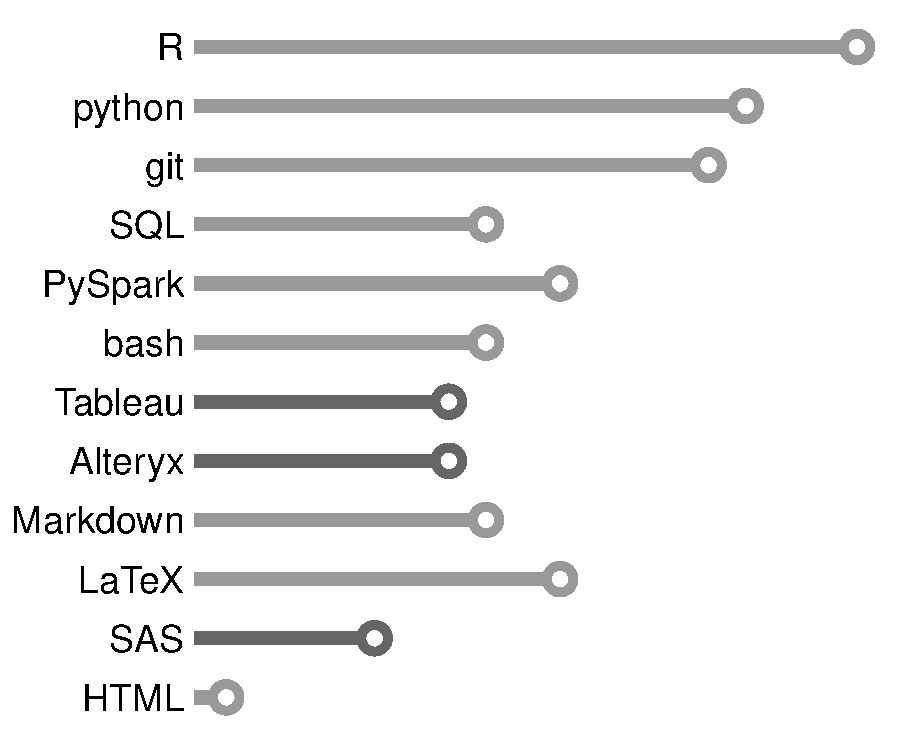
\includegraphics{Ava_Hoffman_Resume-skills_plot}

	\normalsize \toolboxitem{lightgray}{statistics} \\ \footnotesize
	Bayesian methods (RStan) $\cdot$
	hierarchical models $\cdot$
	mixture models $\cdot$
	multivariate statistics $\cdot$
	ANOVA $\cdot$
	MANOVA $\cdot$
	PERMANOVA $\cdot$
	dimensionality reduction $\cdot$
	repeated measures \\
	
  \vspace{-6mm} 
  \normalsize \toolboxitem{lightgray}{supervised learning} \\ \footnotesize
  large language model APIs $\cdot$
  random forest $\cdot$
  time series $\cdot$
  linear, nonlinear, logistic regression $\cdot$
  LDA $\cdot$
  SEM \\

  \vspace{-6mm} 
  \normalsize \toolboxitem{lightgray}{unsupervised learning} \\ \footnotesize
  PCA $\cdot$
  NMDS $\cdot$
  k-means / hierarchical clustering $\cdot$
  feature engineering
}

%----------------------------------------------------------------------------------------
%	 ACHIEVEMENTS
%----------------------------------------------------------------------------------------
\addachievements{
        % \achievementitem{Sustainability Leadership Fellow}{2017-2018}{Colorado State University}{
        % {
\includegraphics[width=\logosize, height=\logosize]{csu}} % logo
        % } % 25\% acceptance rate
        % \achievementitem{Vice President for Research Fellow}{2016-2017}{Colorado State University}{
        % {
\includegraphics[width=\logosize, height=\logosize]{csu}} % logo
        % } % <10\% acceptance rate
        \achievementitem{Excellence in Teaching Award}{2022 (2x), 2023 (2x), 2024 (2x)}{Johns Hopkins University}{
        {
\includegraphics[width=\logosize, height=\logosize]{jhu}} % logo
        }
        \achievementitem{29 peer-reviewed publications}{2010-2024}{\textcolor{special}{\href{https://scholar.google.com/citations?user=k6RyLHsAAAAJ&hl=en}{Google Scholar}}}{
        \faBook % logo
        }
}

%----------------------------------------------------------------------------------------
%	 EXPERIENCE
%----------------------------------------------------------------------------------------
\addexperience{

        \experienceitem{Fred Hutch Cancer Center}{Senior Staff Scientist}{07/2022 - present}{Seattle, WA (remote)}{

          \item Built outreach software for publishing content, previewing data, and helping scientists comply with NIH policies using Shiny, GitHub Actions, and other tools
          \item Co-lead, analyzed, and curated data for \textcolor{special}{\href{https://biodigs.org}{BioDIGS}}, a soil microbe genetics research consortium of over 100 students and faculty 
          \item Co-lead outreach and user research for the NIH \textcolor{special}{\href{https://anvilproject.org}{AnVIL Platform}}, enabling genomic data science via cloud computing for 500+ users
          \item Led and managed \$579k NIH-funded program (\textcolor{special}{\href{https://genomicseducation.org}{"GEMs"}}) that designs open-source genomic data science training modules with under-resourced colleges
          \item Led, developed, and managed \$200k/yr \textcolor{special}{\href{https://daseh.org}{Data Science for Environmental Health program}}, educating ~40 trainees and public health government professionals annually
          \item Taught graduate-level courses in R programming and community data science consulting
          \item \textit{Note that this work was conducted at Johns Hopkins University from 05/2021 - 06/2022.}
       }{hutch} \\
       \vspace{1mm}

       \experienceitem{Johns Hopkins University}{Postdoctoral Fellow}{03/2020 - 05/2020}{Baltimore, MD}{
          \item Used bioinformatic tools to quantify genomic patterns among 1000+ plants adapted to 6 city landscapes
       }{jhu} \\
       \vspace{1mm}
       
       \experienceitem{Boston Consulting Group}{Data Scientist}{03/2019 - 03/2020}{Boston, MA}{
           \item Productionalized PySpark pipeline describing and modeling client's 20K+ commercial banking customers for better product recommendations \& risk intervention
           \item Designed \& hosted fully customized RShiny dashboard for reducing internal carbon emissions by 30\% in 5 years
        }{gamma} \\
        \vspace{1mm}
        
        \experienceitem{Colorado State University}{USDA NIFA Fellow}{01/2017 - 12/2018}{Fort Collins, CO}{
        \item Led the Blue Grama Diversity Project, implementing hierarchical Bayesian models and analyzing 9,000+ genomic features to understand plant traits from population genetics
        }{nifa} \\
      
      
      
%--------------------
%	 EXPERIENCE Plot
%--------------------

% \setkeys{Gin}{width=4in}
% 
% <<experience_plot, echo=FALSE, warning=FALSE, message=FALSE, fig=TRUE, height=3, fig.align='center'>>=
% source("experience_breakdown.R")
% print(experience_plot)
% @
% 
%       \vspace{-40mm}
}

\cheekyfooter{Résumé built using \textcolor{special}{\href{https://github.com/avahoffman/CV-and-resumes}{LaTeX and R}} \today.}

%%%%%%%%%%%%%%%%%%%%%%%%%%%%%%%%%%%%%%%%
\end{document} 
